\subsection{Initial occupations} \label{chap2-initial}

We start by estimating the impact of parental income on the child's first-period occupations, before considering the occupation of mature individuals in the next section. We estimate equation \eqref{chap2-eq:emp-multi1} and report the results in the appendix, those for the binomial logits are reported in Table \ref{chap2-tab:occ-bi1-base} and the multinomial results in Table \ref{chap2-tab:occ-multi1-base}.  Logit coefficients are hard to interpret, hence to visualize the results Figure \ref{chap2-fig:occ-multi1-pinc} displays the probability to be in each occupation when young as a function of parental income.
\begin{figure}[!tb]
    \centering
    \caption{First-period occupation probability according to parental income}
    \label{chap2-fig:occ-multi1-pinc}
    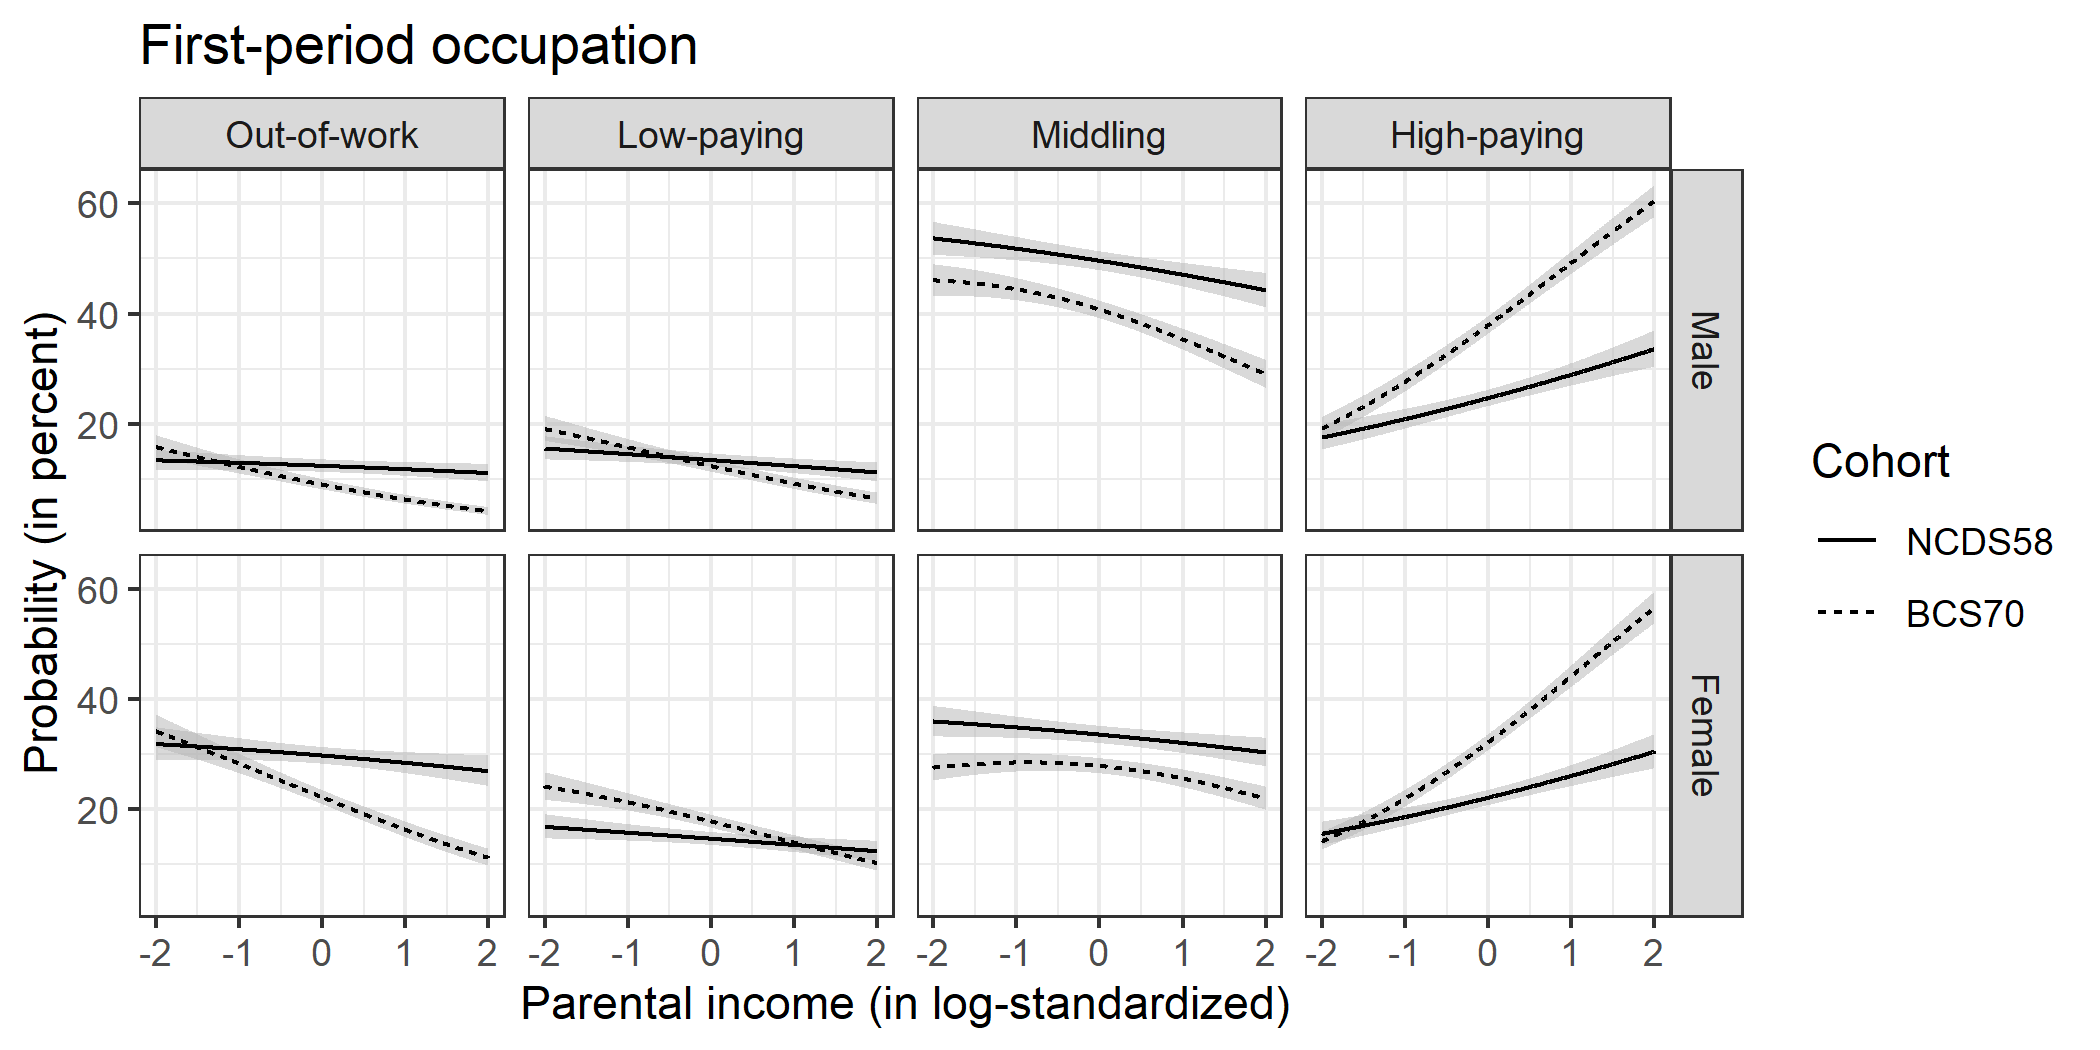
\includegraphics[width=\linewidth]{chap2/graphic/occ-multi1-pinc.png}
    \vspace{-3em}
	\justify\singlespacing\footnotesize{\textit{Notes:} This figure presents the probability, expressed in percent, of being in each type of occupation (out-of-work, low-paying, middling, high-paying) in first period according to parental income, in log-standardized.
	Probabilities are computed for males and females in both cohorts according to the multinomial logistic regression reported in Table \ref{chap2-tab:occ-multi1-base} in the appendix.}
\end{figure}
The probabilities are computed according to the multinomial logistic regression, but the results are qualitatively equivalent when using the binomial estimates. The probabilities are reported separately for the two cohorts and for the two genders; the four columns depict the four possible outcomes, starting with out-of-work occupations on the left.

Consider first the outcomes for the 1958 cohort, depicted by the continuous lines. Parental income is a key determinant of initial occupation, with high income increasing the probability to be in a high-paying occupation and reducing that of being in a middling or low-paying one. There is no effect on the probability of being out-of-work (see also Table \ref{chap2-tab:occ-bi1-base}), a result that is not surprising given the various outcomes included in this category. Note also that the effect of family background is particularly large for high-paying occupations. The levels vary across men and women, with women being more likely than men to be out-of-work and less likely to be in any of the three types of employment.

The impact of parental income on the various probabilities for the 1970 cohort are depicted by the dashed lines. Starting with men, Table \ref{chap2-tab:occ-multi1-base} reports large changes across cohorts in the coefficients on the direct effect of parental income, which are captured in the figures. For example, the coefficient doubles for high-paying occupations, increasing from 0.21 to 0.41, a result that is reflected in the large increase in the slope of the schedule that we observe in the two right panels. There are various possible explanations for this. Obviously, the effect could be operating through education which has become more dependent on parental background (see Appendix \ref{chap2-app-education} for a discussion). Other explanations are that non-cognitive skills have become more important and that they are positively associated with the household’s income, or parental income could be a proxy for the child’s social network, either its size or ‘quality’, which in turn has become more important in determining access to jobs.\footnote{For example, \cite{Blanden2007Accounting}, using the same data as us, show a strengthening of the relationship between parental income and non-cognitive skills between both cohorts. \cite{Major2018Social} emphasize the changing role of education and the increasing importance of the "extra-investments" made by upper-middle class families. For the US, \cite{Chetty2014Land} show that neighborhood characteristics are extensively correlated with mobility.}

As expected, the probability of being in a middling occupation has fallen for all individuals, irrespective of family background. The decline has been greater the higher parental income is. Together with the previous result this indicates that as the share of high-paying jobs increased, those from high-income households are more likely to go into high-paying jobs at the expense of middling ones. The probability of being in a low-paying occupation has pivoted around the mean, with those at the bottom (resp. top) of the parental income distribution being more (resp. less) likely to be in that occupation in the 1970 than in the 1958 cohort. The schedule for being out of work displays a steeper slope, with a decline in the probability of being in this category for all men except those at the very bottom of the parental income distribution.

Consider now the schedules for women. Starting from the right, we can see that women experienced a large decline in the likelihood of being out-of-work, consistent with the increase in female labour force participation observed over the period. Yet, the reduction is strongly correlated to parental income, even more so than for men. The probability of being in a low-paying occupation has increased at virtually all points of the distribution---except at the very top---indicating that much of the increase in female participation occurred through access to low-paying jobs. The probability of being in middling occupations has declined for the younger cohort, as is the case for men. Interestingly, for women the schedule is non-monotonic. At the bottom of the parental income distribution, an increase be income raises the probability of being in middle occupations, with the effect then turning negative. This seems to indicate that in the lower segment of the parental income distribution, an increase in income confers women a occupational advantage, allowing them to access middling rather than low-paying jobs. As is the case for men, the slope of the schedule for high-paying occupations has increased sharply across the two cohorts.

These patterns indicate that parental income conferred a greater advantage for those born in 1970 as compared to those born in 1958. Much of the change was driven by reduced entry into middling occupations, which was offset by a greater likelihood to in in a high-paying (resp. low-paying) occupation for those coming from households at the top (resp. bottom) of the parental income distribution.

\subsection{Mature occupations} \label{chap2-mature}

We turn now to the probability of being in occupation $k$ at age 42. Recall that we suppose that as well as depending on parental income, the occupation of mature workers depends on their job at the start of their career. We hence consider both an expression that does not include the effect of initial occupations, as given by equation \eqref{chap2-eq:emp-multi2}, and one in which they are included, as in equation \eqref{chap2-eq:emp-multi3}. The former specification is equivalent to those usually found in the literature.

As before, we estimate this equation both separately for the four occupations as well as in a multinomial regression. The full results are reported in Tables \ref{chap2-tab:occ-multi23-base} and \ref{chap2-tab:occ-bi23-base} in the appendix, while Table \ref{chap2-tab:occ-multi2-short} summarizes the multinomial results for the baseline regression, in which we do not consider the effect of initial occupations.
\begin{table}[!tb]
    \centering
    \caption{Second-period occupation probability}
    \label{chap2-tab:occ-multi2-short}
    \begin{threeparttable}
        \setlength{\tabcolsep}{18pt}
        \begin{tabular}{l D{.}{.}{5.3} D{.}{.}{5.5} D{.}{.}{5.5}}
\toprule
 & \multicolumn{3}{c}{Multinom. logit - Dep. var.: Second-period occ.} \\
\cmidrule(lr){2-4}
 & \multicolumn{1}{c}{Low-paying} & \multicolumn{1}{c}{Middling} & \multicolumn{1}{c}{High-paying} \\
\midrule
Par. inc.              & 0.01   & 0.04       & 0.19^{***} \\
                       & (0.04) & (0.04)     & (0.04)     \\
Par. inc. $\times$ BCS & 0.05   & 0.15^{***} & 0.36^{***} \\
                       & (0.06) & (0.05)     & (0.05)     \\
\midrule
Num. obs. & \multicolumn{1}{c}{14763} & \multicolumn{1}{c}{14763} & \multicolumn{1}{c}{14763}\\
\bottomrule
\end{tabular}

        \begin{tablenotes}[flushleft]
            \footnotesize{\item\textit{Notes}: 
            % Stars and SE
            $^{***}p<0.01$; $^{**}p<0.05$; $^{*}p<0.1$. Standard errors between parentheses. 
            % Baseline outcome
            Out-of-work occupation in second period is the base outcome of the multinomial logistic regression.
            % Referent group
            Male in the NCDS58 cohort in out-of-work occupation in first period is the referent group. 
            % Variables details
            Parental income in logarithm and then standardized at the cohort level. 
            % Control variables
            Control variables in all regressions include Intercept, BCS cohort, Female and Female $\times$ BCS; see Table \ref{chap2-tab:occ-multi23-base} in the appendix for these coefficients.}
        \end{tablenotes}
    \end{threeparttable}
\end{table}

As before, the reference category are those out of work. Parental income has a large impact on occupational outcomes at age 42, with the coefficient for high-paying jobs almost doubling across cohorts. This result is in line with the extensive work that has found an increased correlation in parent-child incomes, as discussed in the introduction. While a one-standard-deviation increase in parental income used to raise the odds to be in a high-paying occupation by 21\% for the older cohort, this same increase raises the odds by 73\% for the younger one.\footnote{These coefficients are obtained by taking the exponential of the change in log odds, i.e. $\exp(0.19) = 1.209$ and $\exp(0.19+0.36) = 1.733$.} 

To illustrate the relationship between parental income and occupational dynamics, Figure \ref{chap2-fig:occ-multi2-pinc} reports the probabilities of being in each occupational category at age 42 as a function of parental income, for both genders.
\begin{figure}[!tb]
    \centering
    \caption{Second-period occupation probability according to parental income}
    \label{chap2-fig:occ-multi2-pinc}
    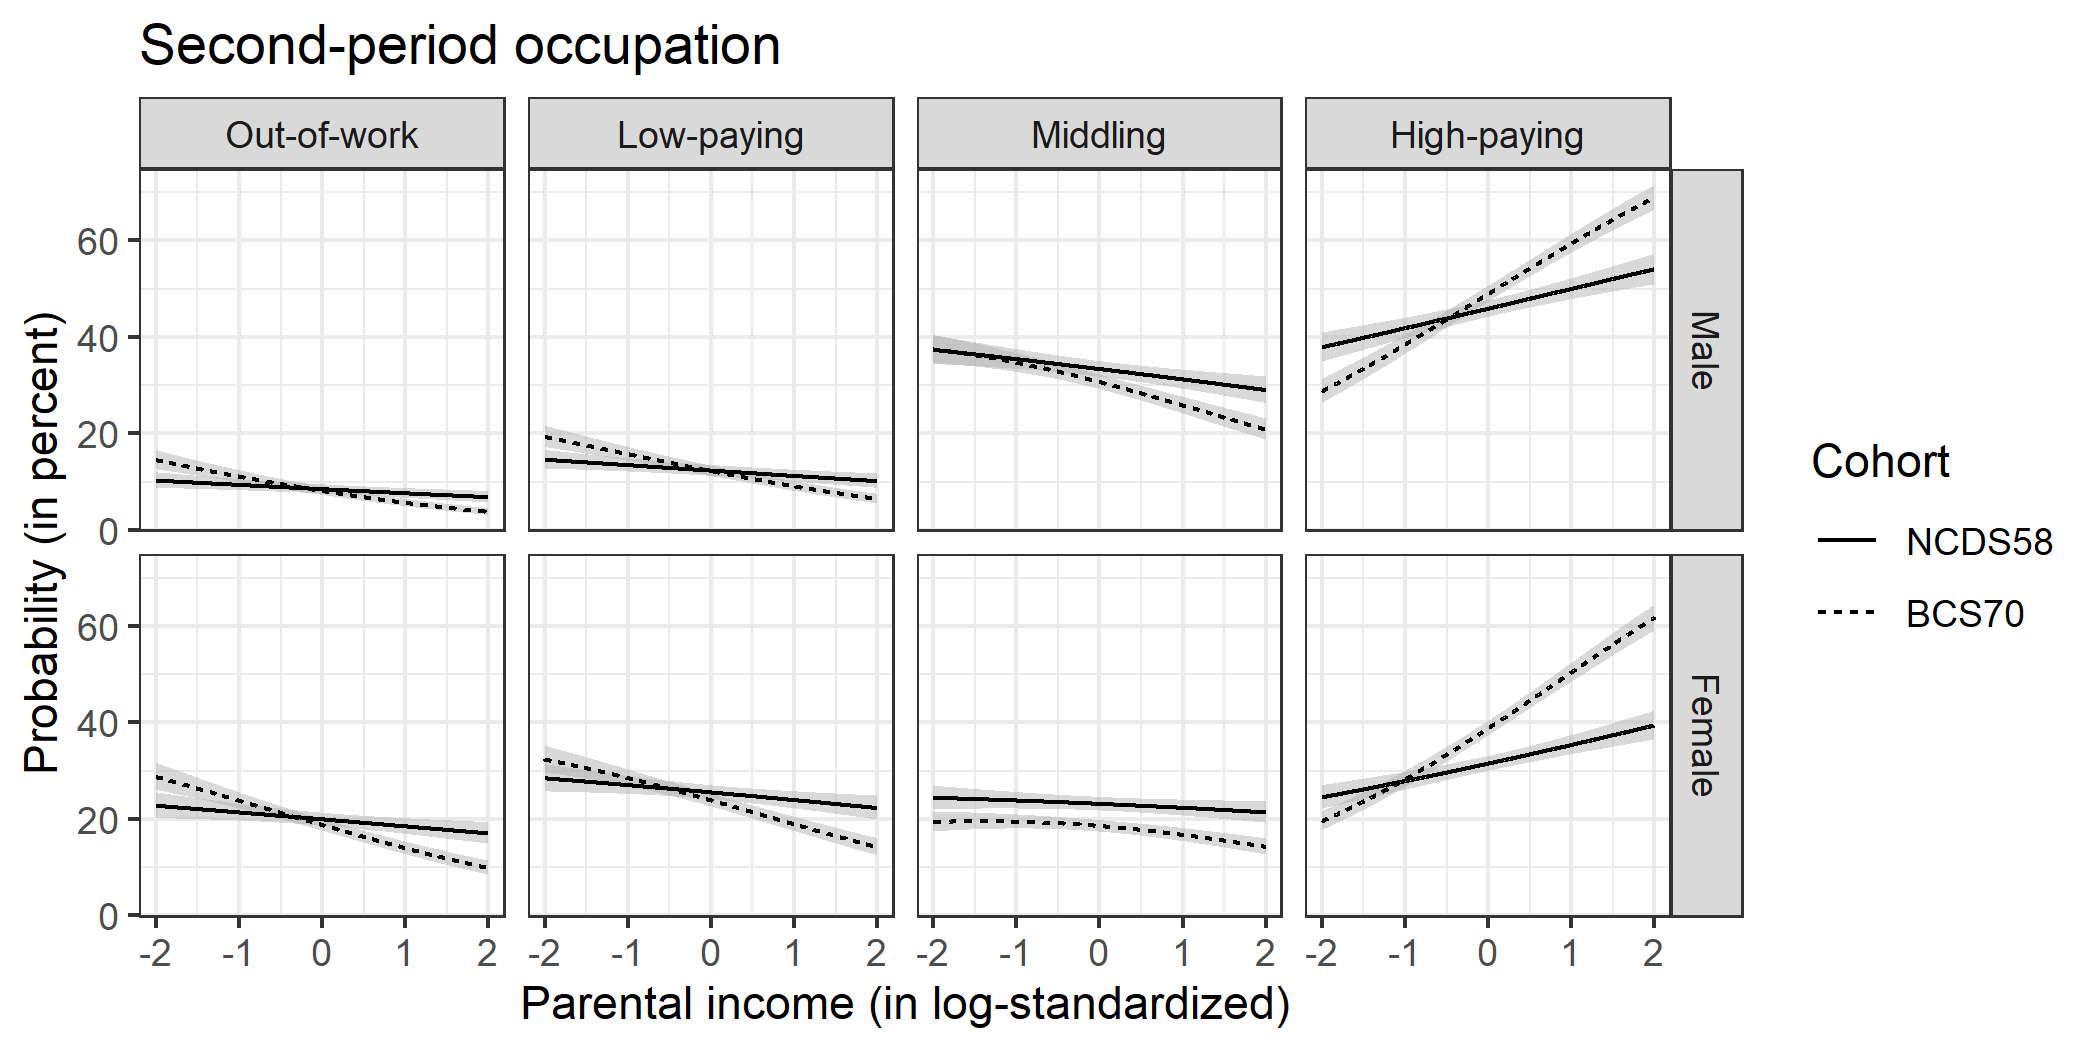
\includegraphics[width=\linewidth]{chap2/graphic/occ-multi2-pinc.png}
    \vspace{-3em}
	\justify\singlespacing\footnotesize{\textit{Notes:} This figure presents the probability, expressed in percent, of being in each type of occupation (out-of-work, low-paying, middling, high-paying) in second period according to parental income, in log-standardized.
	Probabilities are computed for males and females in both cohorts according to the multinomial logistic regression reported in Table \ref{chap2-tab:occ-multi23-base} in the appendix.}
\end{figure}
As for initial occupations, coming from a better-off background increases the probability of being in a high-paying occupation and reduces all others. The main difference with our results for initial occupations is the crossing of several of the probability schedules. Consider the probability of being in a high-paying occupation; we can ask whether individuals from all backgrounds have benefited from the increase in the share of such jobs across the two cohorts. Figure \ref{chap2-fig:occ-multi1-pinc} indicates that, as far as initial occupations are concerned, this is the case, with even those men at the bottom of the parental-income distribution (i.e. 2 standard deviations below the average) exhibiting a larger probability of being in a high-paying job for the younger than for the older cohort. In contrast, we can see in Figure \ref{chap2-fig:occ-multi2-pinc} that by age 42 only those from sufficiently well-off households have reaped the benefits of the expansion in high-paying jobs. Men whose parents had an income 0.5 standard-deviations below the average had the same probability of being in a high-paying occupation in both cohorts; those with lower parental income, experienced a lower probability if born in 1970 than if born in 1958.

Figure \ref{chap2-fig:occ-multi2-pinc} is reminiscent of the analysis in \cite{Major2018Social}, who show, using the same data, that the effect of parental income on the probabilities of being in the various quintiles of the income distribution has increased across the two cohorts (see \cite{Major2018Social}, Figures 0.1 and 0.2). Our results indicate, not surprisingly, that the occupational structure is behind the observed changes in income mobility and closely mimic their findings when we consider the probabilities of being in each of the four occupations for each decile in the parental-income distribution (see Figure \ref{chap2-fig:occ-multi2-quant-male} in Appendix \ref{chap2-app-additional}).


\subsection{From initial to mature occupations} \label{chap2-intra}

The marked change in the overall effect of parental income across the two generations can be due to changes in either how parental income impacts initial occupations or in its effect on mobility during the child's career, i.e. on intra-generational mobility. As we have seen above, the influence of parental background on the former has become stronger; we turn next to whether coming from a better-off background also changes the extent to which, given her initial occupation, an individual progresses over her career.

Table \ref{chap2-tab:occ-multi23-base} in Appendix \ref{chap2-app-logit} reports the multinomial results when we introduce initial occupations in the regressions for occupation at 42 and we provide a graphical analysis in Figure \ref{chap2-fig:occ-multi3-pinc-male}. The figure displays the difference, expressed in percentage points, in the probability of being in each second-period occupation (out-of-work, low-paying, middling, high-paying) conditional on first-period occupation between the BCS70 and the NCDS58 cohorts. 
\begin{figure}[!tb]
    \centering
    \caption{Change in second-period occupation probability conditional on first-period occupation and parental income (male only)}
    \label{chap2-fig:occ-multi3-pinc-male}
    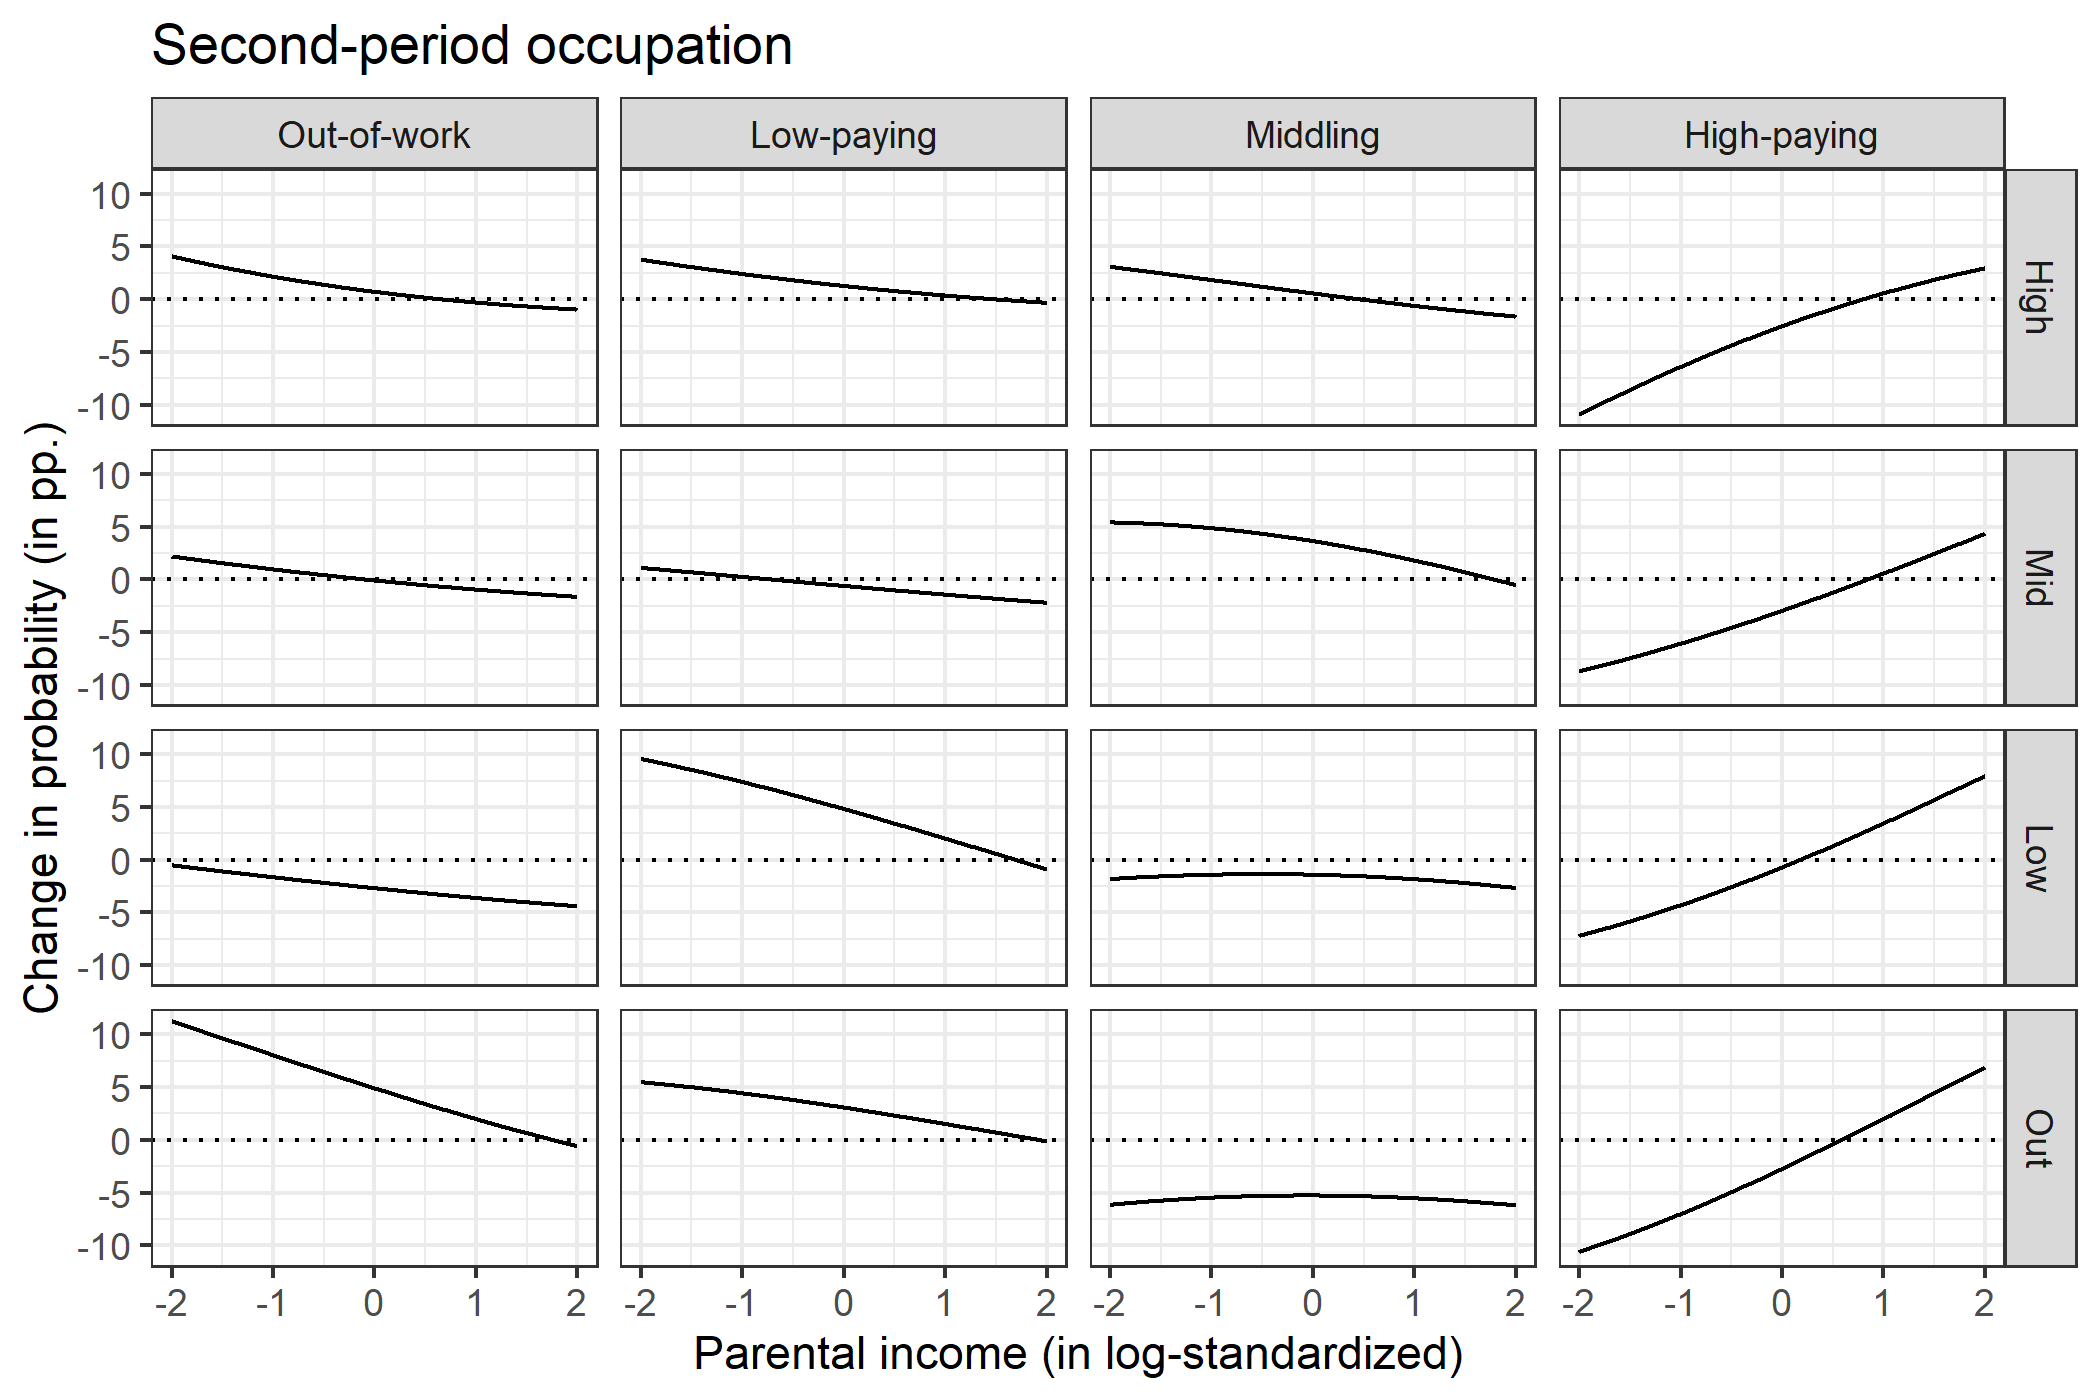
\includegraphics[width=\linewidth]{chap2/graphic/occ-multi3-pinc-male.png}
    \vspace{-3em}
    \justify\singlespacing\footnotesize{\textit{Notes:} This figure presents the difference, expressed in percentage points, between the BCS70 and the NCDS58 cohorts in terms of probability of being in each type of second-period occupation (out-of-work, low-paying, middling, high-paying), conditional on the first-period occupation, according to parental income, in log-standardized.
    Probabilities are computed for males in both cohorts according to the multinomial logistic regression reported in columns (2) of Table \ref{chap2-tab:occ-multi23-base}}
\end{figure}
Each panel represents the gap across cohorts in a particular transition probability for various levels of (standardized) parental income, with positive values implying that the younger cohort has a greater probability of moving from occupation $j$ to occupation $k$, and vice versa. The reported changes are those for men, with the equivalent figure for women provided in appendix \ref{chap2-app-additional}---see Figure \ref{chap2-fig:occ-multi3-pinc-female}.

Consider first individuals at the mean of the distribution. The probability of being in a middling occupation in late career has increased by almost 3.7 pp. for those who started in such occupation but declined for those starting in low-paying occupations or out of work. This indicates a reduction in upwards mobility for those starting in the least well-paid categories. For example, for those who were initially out-of-work, the probability of remaining there has increased by 4.92 pp., and although the probability of being in a high-paying occupation at 42 has slightly increased (by 0.71 pp.), this has occurred at the expense of a large decline in the likelihood of moving into low-paying or middling jobs. The fourth column of graphs, reporting changes in the probability of being in a high-paying occupation, indicates that---for those with mean parental income---the probability of being in such an occupation has fallen irrespective of the initial job. The change is small for those starting in low-paying occupations (-0.71 pp.) but larger for the other three initial occupations, with values between -2.5 and -2.9 pp. This is a surprising finding given that the share of such jobs rose by 5.4 pp.

These changes hide large differences depending on parental background. Consider the changes in the probability of being in a high-paying occupation across cohorts. For those at the top and the bottom of the parental income distribution the changes are large and of opposite sign. Notably, for those who came from a household with parental income 2-standard-deviations below the mean there is a reduction in the probability of attaining the top occupations, irrespective of the initial occupation, which is of considerable magnitude, between 7.2 and 11 pp.. Note that even those who started in high-paying occupations are now less likely to remain there if parental income is low. In contrast, when parental income is 2-standard-deviations above the mean, there is an increase in the likelihood of remaining in or moving to the top, with those who started in a low-paying occupation experiencing a particularly large increase, by 8 pp. 

The second important pattern observed in the data is a dichotomy that appears for those who started in a low-paying occupation. Their probability of moving to a middling occupation has fallen, but the alternative outcome depends on parental income. For those at the bottom of the distribution, the likelihood of remaining in a low-paying occupation has increased (by  4.8 pp. for those with average parental income and by 9.6 pp. for those at -2 standard deviations). In contrast, for those at the top of the parental income distribution the decline in mobility into middling jobs has been accompanied by a greater probability of moving into a high-paying occupation. The natural progression in which individuals would move from low-paying into middling occupations as their careers evolved seems to have weakened, and has been replaced by higher probabilities of either staying in the occupation of origin or jumping up to a high-paying one, with the transition probabilities being strongly dependent on parental income. An equivalent pattern is found when considering those who started in middling occupations, with those at the top (bottom) of the parental income distribution being more likely to be in high-paying (low-paying) jobs in the younger than in the older cohort. 

\subsection{Intra-generational mobility and parental income}

In order to provide a compact measure of mobility, we define three possible outcomes for the second period. Downward mobility is defined as ending up in a category with lower average pay than the individual's initial category; persistence consists of remaining in the same category, and upwards mobility occurs when the individual moves to a category with higher average pay. Hence for those starting in a low-paying occupation, downward mobility occurs if they are out-of-work at age 42, and upwards mobility if they are in a middling or high-paying occupation. 

The upwards/downwards intra-generational mobility measures are depicted graphically in Figure \ref{chap2-fig:persist-both}, in which we plot the \emph{change} in the three probabilities (of moving up, remaining in, and moving down with respect to the initial occupation) for different deciles of the parental income distribution; see also Table \ref{chap2-tab:mob-pinc-both} in the appendix.
\begin{figure}[!tb]
    \centering
    \caption{Change in intra-generational mobility across cohorts}
    \label{chap2-fig:persist-both}
    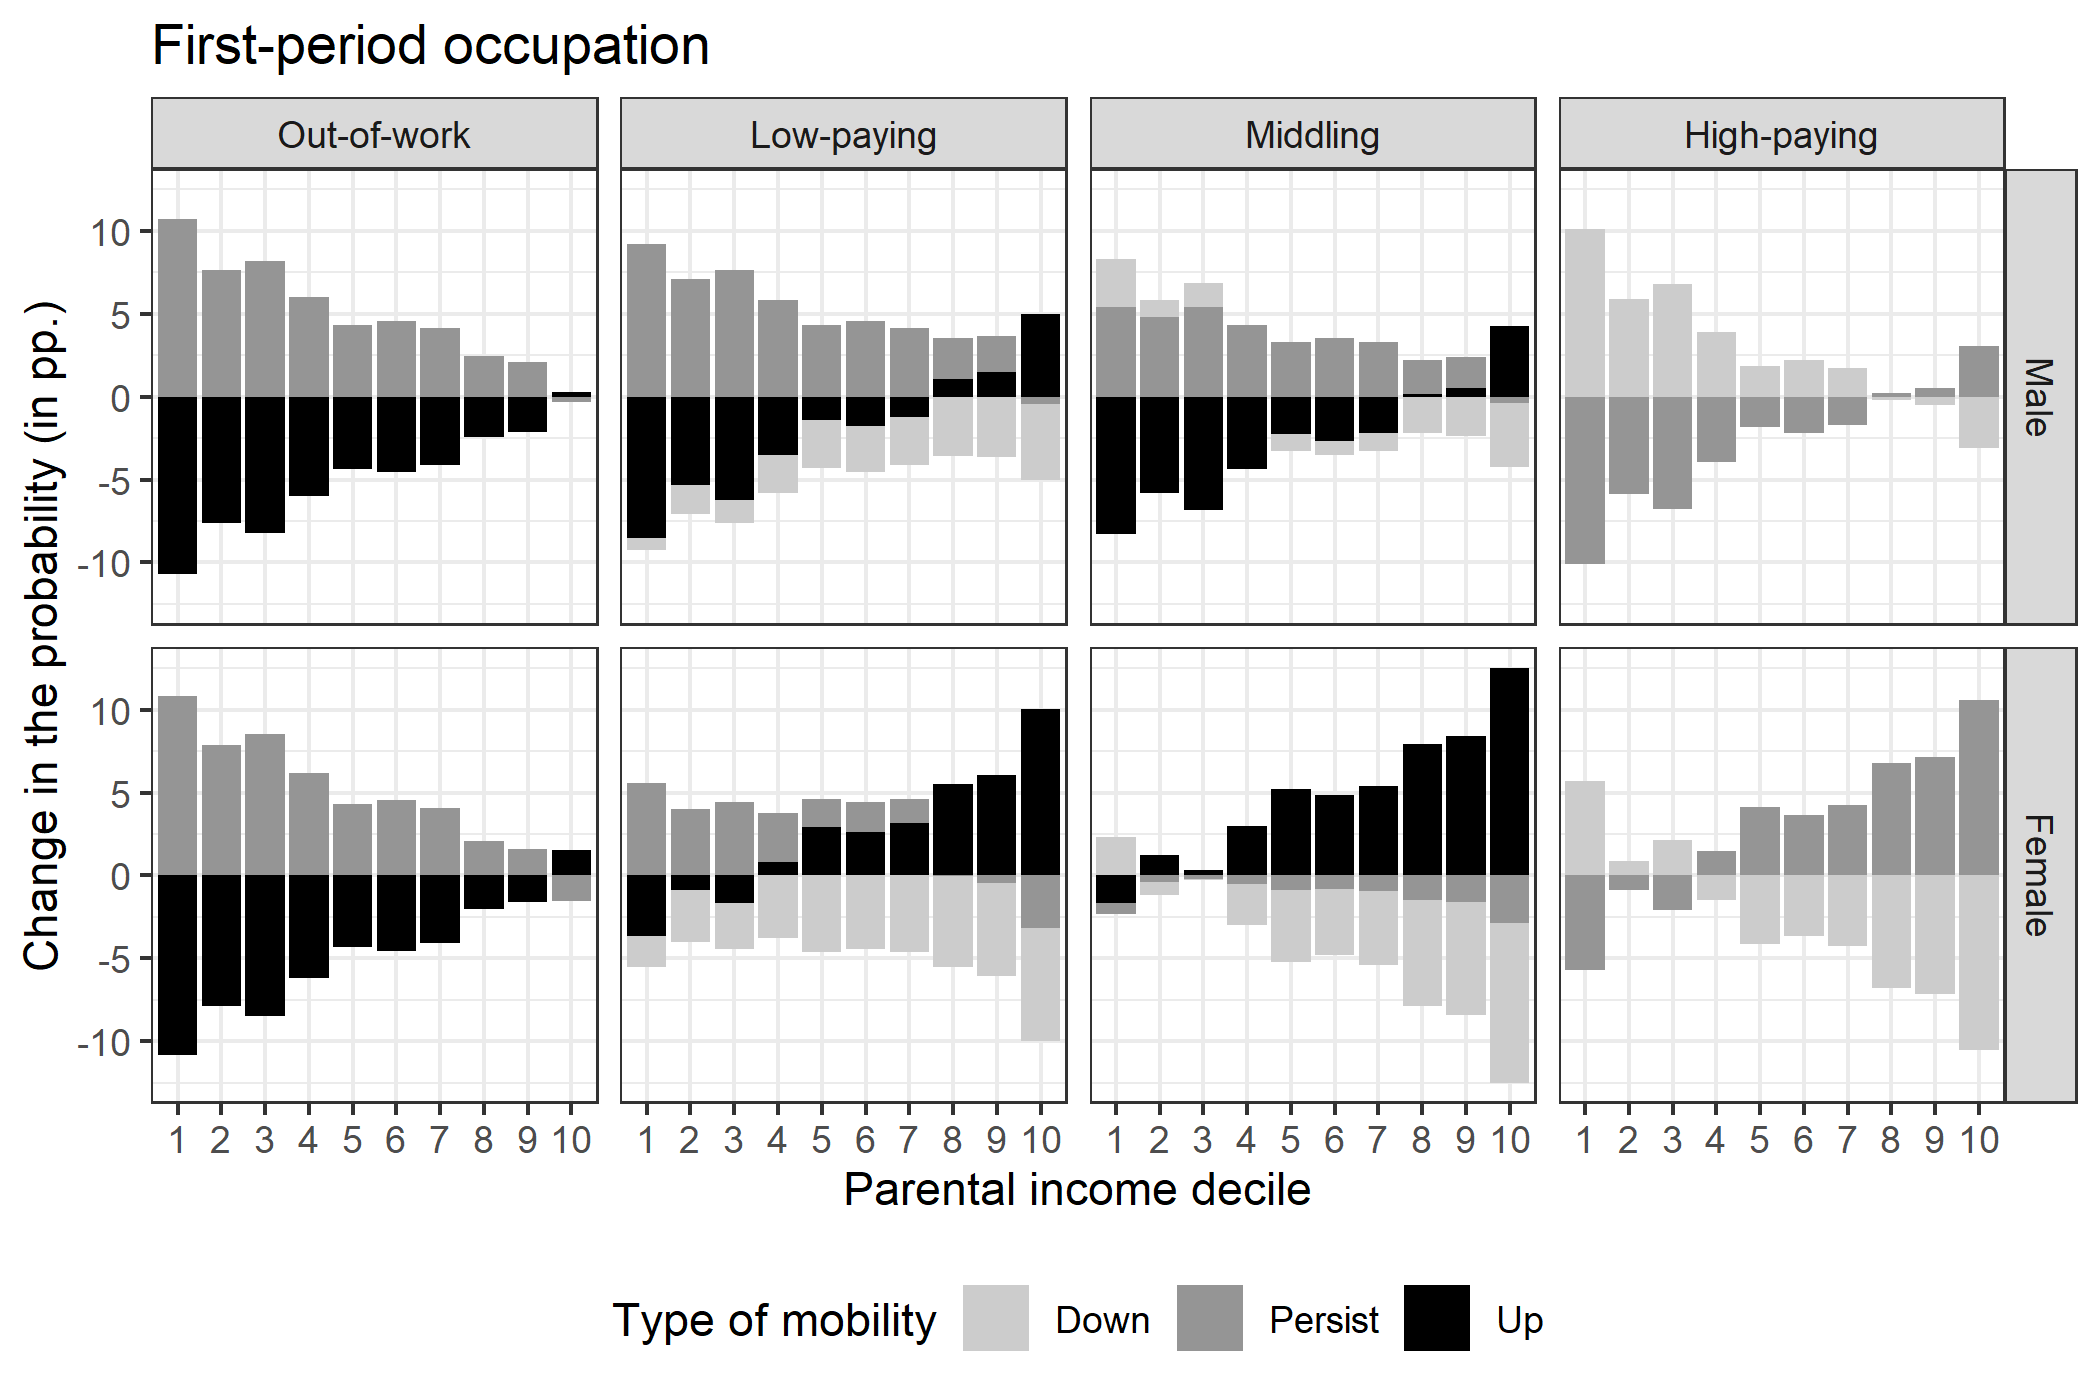
\includegraphics[width=\linewidth]{chap2/graphic/persist-both.png}
    \vspace{-3em}
    \justify\singlespacing\footnotesize{\textit{Notes:} This figure presents the difference, expressed in percentage points, between the BCS70 and the NCDS58 cohorts in terms of type of mobility (down, persist, up) conditional on the first period occupation (out-of-work, low-paying, middling, high-paying) according to the decile of the parental income distribution.
    Probabilities are computed for males and females at each parental income decile, according to the multinomial logistic regression reported in columns (2) of Table \ref{chap2-tab:occ-multi23-base} in the appendix.}
\end{figure}

Consider first those who started in high-paying occupations. The two possible occupational dynamics are to move downwards (depicted in light grey) or to remain in a high-paying occupation (depicted in dark grey). Those born to parents in the top decile are 3 pp. more likely to stay in that occupation and 3 pp. less likely to move into a lower-income occupation in the 1970 cohort than those born in 1958. The reverse effect appears for those at the bottom of the parental income distribution, with those in the bottom decile being 10 pp. more (less) likely to experience downwards mobility (remain in the occupation). The reduction in persistence falls as we move up the parental income distribution, with the sign reversing for the 9th and 10th deciles. The figure displays what we could call a \emph{polarization of mobility}, whereby for those in the middle of the distribution there have been only moderate changes in mobility, while at the extreme the changes have been large, although in opposite directions for those at the bottom and at the top. 

An equivalent pattern is observed for those that start their careers in middling occupations. Those at the bottom of the parental distribution witnessed sharp declines in upwards mobility and higher persistence and likelihood of moving down, with the size of the changes declining as we move along the income distribution. The pattern is reversed from the 8th decile, with the likelihood of moving upwards increasing across cohorts for the top three deciles. The polarization of mobility is also apparent for those starting in low-paying occupations for whom the probability of moving into middling or high-paying occupations increases only for the top three deciles. Lastly, for those initially out-of-work, only those in the top decile of the parental income distribution witness an increase in the likelihood of upwards mobility. Note that for those in the bottom decile the magnitudes of the change are large: the probability of staying has increased by 10 pp., which is offset by an equivalent decline in the probability of moving upwards. Overall these results indicate that the change in the structure of employment has been accompanied by a polarization of intra-generational mobility, with the probabilities of moving across occupations changing in opposite directions depending on whether individuals had parents at the top or at the bottom of the income distribution.

Not surprisingly, the dynamics for women differ considerably from those for men, as women of the older cohort where much less likely to occupy middling and especially high-paying occupations. The bottom panels of Figure \ref{chap2-fig:persist-both} capture, however, the advantage that parental income gives in providing the means for upwards mobility. Irrespective of parental income, women starting in a high-paying occupation (resp. middling) have a greater probability of remaining there (moving upwards) for the younger cohort. This is not surprising in view of the occupational upgrading experienced by women of the younger cohort. In contrast, for those who started in low-paying occupations, a polarization appears, although the turning point occurs for lower parental incomes than in the case of men (4th decile), indicating the tension between the general occupational upgrading of women and the decline in mobility observed for workers coming from a less well-off background. The results for those out of work broadly mimic those for men. Overall, despite the differences due to women's increased access to all occupations, these figures confirm the increased importance of parental income for intra-generational mobility.

